\documentclass[a4paper,10pt]{jsarticle}
\usepackage{graphicx}
\usepackage{robo}

\title{ロボット実験1 報告書}

\begin{document}

	\section{オームの法則の確認実験}
		\subsection{実験目的}
		オームの法則は,  電気回路を解析する際の最も基本的かつ重要な法則のひとつである.  本実験では, 可変抵抗器を用いた電気回路において,  オームの法則が成り立つことを確認する.
		\subsection{オームの法則}
		導体中の2点間の電位差$E [V]$は,  その2点間を流れる電流$I[A]$に比例する.  すなわち,  比例定数$R$とすると,  式1.1 のように表される.
			\begin{equation}
				E = I R
				\label{:eq:ohm}
			\end{equation}
			
		このような電流と電位差の関係を,  オームの法則(Ohm's law) と呼ぶ.  比例定数$R [\Omega]$は,  導体の形状や電気的特性によって決まり,  電気抵抗と呼ばれる.
		\subsection{実験方法}
			本実験において使用した実験機器を表1.1に示す.  ディジタルマルチメータは,  電流および電圧測定のために2個用いた.
			\begin{table}[h]
			\caption{使用した実験器具}
				\label{equip}
				\begin{center}
				\begin{tabular}{|c|c|c|}\hline
				機器名 & メーカ & 型番 \\ \hline
				直流安定化電源 & A社 & DPS-10 \\ \hline
				ディジタルマルチメータ & B社 & DM-55 \\ \hline
				\end{tabular}
				\end{center}
			\end{table}
			
			図1.1に,  実験回路の構成を示す.  可変抵抗器に直流電源を接続する.  可変抵抗器の両端の電位差,  および回路を流れる電流を,  それぞれディジタルマルチメータを用いて計測する.
			
			\begin{figure}[h]
			\begin{center}
			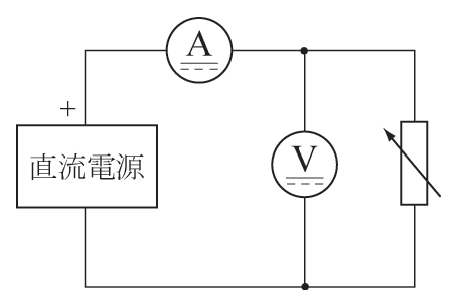
\includegraphics[width=5cm]{circuit.eps}
			\end{center}
			\caption[]{実験回路. }
			\label{circuit}
			\end{figure}
			
			実験は次の手順で行った.
			
			\begin{enumerate}
			\item 可変抵抗器の抵抗値を $100[\Omega]$に合わせる.
			\item 直流電源の出力電圧を $0[V]$から$5[V]$まで,  $1[V]$ごとに変化させながら,  電圧計および電流計の値を記録する.
			\item 可変抵抗器の抵抗を $500[\Omega]$に合わせ,  上記と同様に電圧,  電流値を記録する.
			\end{enumerate}
			
		\subsection{実験結果}
			表1.2に,  可変抵抗器の抵抗値$R[\Omega]$が,  $100 [\Omega]$および$500 [\Omega]$のときの,  可変抵抗器の電圧 $e[V]$ と 電流$i[mA]$ の計測値を示す.  また,  図1.2に,  そのグラフを示す.
			\begin{table}[h]
			\caption{電圧と電流の関係}
				\label{relation}
				\begin{center}
				\begin{tabular}{|c|c|c|}\hline
				電圧 $e[V]$ & 電流 $i[mA] (R = 100 [\Omega]$) & 電流 $i[mA] (R = 500 [\Omega]$)  \\ \hline
				0 & 0 & 0 \\ \hline
				1.0 & 9.92 & 1.99 \\ \hline
				2.0 & 19.8 & 4.01 \\ \hline
				3.0 & 29.7 & 5.98 \\ \hline
				4.0 & 39.5 & 7.99 \\ \hline
				5.0 & 49.5 & 9.97 \\ \hline
				\end{tabular}
				\end{center}
			\end{table}
			
			\begin{figure}[h]
			\begin{center}
			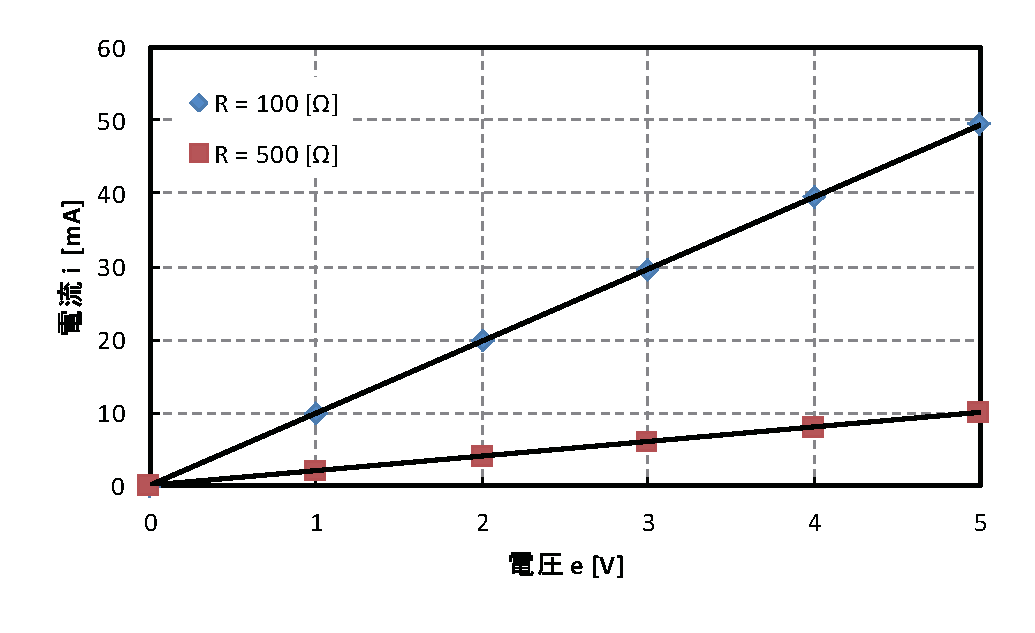
\includegraphics[width=10cm]{ohmu2.eps}
			\end{center}
			\caption[]{電圧と電流の関係. }
			\label{circuit}
			\end{figure}
			
			最小二乗法により求めた図1.2の近似線より,  電流,  電圧の計測値から式1.1.に求められる抵抗値は,  $ R = 100[\Omega], 500 [\Omega] $の場合, それぞれ$101.1[\Omega]$,  $501.3[\Omega]$となった.
			\subsection{考察}
			式1.1より求めた抵抗値と,  実験に用いた抵抗器との抵抗値との間には,  $ R = 100[\Omega], 500[\Omega]$の場合,  それぞれ, $1.1[\Omega], 1.3[\Omega]$の誤差があった.  一般的に, 電源には内部抵抗が存在するため,  これらの誤差の原因は電源の内部抵抗であると考えられる [1].  
			
			
			\begin{thebibliography}{9}
			\bibitem{book1}
			 大熊康弘,  はじめての電気回路,  技術評論社,  2006.
			\end{thebibliography}

\end{document}